% $Id: recountanalysis.tex,v 1.1 2005/07/12 19:29:28 jkatz Exp $
\documentclass[12pt]{article}
\usepackage{graphicx}
\usepackage[dvips, letterpaper, body={6.5in, 9in}, top=1in, left=1in]{geometry}
\usepackage{rotating}
\usepackage{vmargin}
\usepackage{setspace}
\usepackage{hyperref}
\usepackage{supertabular}
\usepackage[table]{xcolor}
\usepackage{amsmath}
\usepackage{amsfonts}

\newcommand{\field}[1]{\mathbb{#1}}


% Vmargin
\setpapersize{USletter}
\setmarginsrb{1in}{1in}{1in}{1in}{0pt}{0mm}{0pt}{0.25in}

\title{PS C236A/ Stat C239A \\ Regression}

\author{Erin Hartman}

\date{September 2, 2009}

\begin{document}

\maketitle



\section{OLS in Matrix Form}

In algebraic notation, the regression model for unit $i$ can be written as:
\[ y_{i} = \beta_{1}x_{i1} + \beta_{2}x_{i2} + \dots + \beta_{k}x_{ik} + \epsilon_{i} \]

Therefore, with $n$ observations, all of the observations can be written as a system of equations:

\[ y_{1} = \beta_{1}x_{11} + \beta_{2}x_{12} + \dots + \beta_{k}x_{1p} + \epsilon_{1} \]
\[ y_{2} = \beta_{1}x_{21} + \beta_{2}x_{22} + \dots + \beta_{k}x_{2p} + \epsilon_{2} \]
\[ \vdots \]
\[ y_{n} = \beta_{1}x_{n1} + \beta_{2}x_{n2} + \dots + \beta_{k}x_{np} + \epsilon_{n} \]

The above system of equations can be expressed in matrix form as:
\[ \left( \begin{array}{c} y_{1} \\  y_{2} \\   \vdots \\  y_{n}  \end{array} \right) =  
\left( \begin{array}{cccc}
x_{11} & x_{12} & \dots & x_{1p} \\
x_{21} & x_{22} & \dots & x_{2p} \\
\vdots & \vdots & \ddots & \vdots \\
x_{n1} & x_{n2} & \dots & x_{np}
\end{array} \right)  \left( \begin{array}{c} \beta_{1} \\  \beta_{2} \\   \vdots \\  \beta_{p}  \end{array} \right)   +  \left( \begin{array}{c} \epsilon_{1} \\  \epsilon_{2} \\   \vdots \\  \epsilon_{n}  \end{array} \right) \]

% from freedman 41
\begin{list}{$\bullet$}{}
\item On the left hand side of the equation, we have $\mathbf{Y}$ which is an $n \times 1$ vector of \emph{observable} random variables, also known as the \emph{dependent} or \emph{response} variable.  Each unit of observation corresponds to a $Y_{i}$
\item On the right hand side is $\mathbf{X}$, an $n \times p$ matrix of \emph{observable} random variables.  $\mathbf{X}$ is also called the \emph{design matrix}.  Each column of $\mathbf{X}$ is a variable, also called \emph{explanatory}, \emph{dependent} variables or \emph{covariates}.  Each row is a unit of observation
\item Next to $\mathbf{X}$ is $\beta$, a $p \times 1$ vector of \emph{parameters}.  These parameters are typically unknown and must be estimated from the data
\item Also on the right hand side is $\mathbf{\epsilon}$, an $n \times 1$ vector of \emph{unobservable} random variables.  $\mathbf{\epsilon}$ is also referred to as the \emph{random error} or \emph{disturbance} term.
\item Note that if we wish to include an intercept, then we simply make the first column of $X$ be a $n \times 1$ vector of 1s
\end{list}

Therefore, we can write the OLS regression equation as such:
\[ Y = X \beta + \epsilon \]

\subsection{Deriving $\hat{\beta}$}

We know:
\[ e = Y - X \beta  \]
Then the sum of squared residuals can be defined as:
\begin{align} e^{T}e &= \sum_{i = 1}^{n} e_{i}^2 \nonumber \\
 &= (Y - X \beta)^{T} (Y - X \beta) \nonumber\\
  &= Y^{T}Y - 2Y^{T}X\beta + \beta X^{T}X \beta \nonumber \end{align} 

Making the first order conditions for $\hat{\beta}$:
\doublespacing
\[ \begin{array}{rrl} & \delta (e^{T}e) / \delta \beta & = 0   \\
\Rightarrow & -2X^{T}Y + 2 X^{T}X\hat{\beta}  & = 0 \\
\Rightarrow & \hat{\beta} &= (X^{T}X)^{-1}X^{T}Y \end{array} \]
\singlespacing

so long as the matrix $X^{T}X$ is invertible.

\subsection{Deriving $\hat{\sigma}^{2}$}

Recall:
\doublespacing
\[ \begin{array}{rrl} & \hat{\beta} &= (X^{T}X)^{-1}X^{T}Y \nonumber \\
& &= (X^{T}X)^{-1}X^{T}(X\beta + \epsilon) \\
\Rightarrow & \hat{\beta} - \beta &= (X^{T}X)^{-1}X^{T} \epsilon
\end{array} \]
\singlespacing


Plugging this into the covariance equation:
\doublespacing
\[ \begin{array}{rl}
cov(\hat{\beta} | X) &= E[(\hat{\beta} - \beta)(\hat{\beta} - \beta)'|X] \\
 &= E\big[ \big((X^{T}X)^{-1}X^{T}\epsilon \big) \big((X^{T}X)^{-1}X^{T}\epsilon)' | X\big] \\
 &= E[ (X^{T}X)^{-1}X^{T} \epsilon \epsilon^{T}X(X^{T}X)^{-1} | X] \\
 &= (X^{T}X)^{-1}X^{T} E(\epsilon\epsilon^{T} | X) X(X^{T}X)^{-1}  \\
 &\qquad \text{where } E(\epsilon\epsilon^{T} | X) = \sigma^{2} I_{p \times p} \\
 &= (X^{T}X)^{-1}X^{T} \sigma^{2} I_{p \times p} X(X^{T}X)^{-1} \\
&= \sigma^{2} (X^{T}X)^{-1}X^{T}X(X^{T}X)^{-1} \\
&= \sigma^{2} (X^{T}X)^{-1}
\end{array} \]
\singlespacing

We estimate $\sigma^2$ dividing the residuals squared by the degrees of freedom because the $e_{i}$ are generally smaller than the $\epsilon_{i}$ due to the fact that $\hat{\beta}$ was chosen to make the sum of square residuals as small as possible.
\[ \hat{\sigma}^2 = \frac{1}{n-p}\sum_{i = 1}^{n} e_{i}^2 \]

\subsection{The Hat Matrix}
The \emph{hat matrix}, or \emph{projection matrix}
\[ H = X(X^{T}X)^{-1}X^{T} \text{ with } \tilde{H} = I - H \]
where $HY$ is the part of $Y$ that projects into $X$.  We use the hat matrix to find the fitted values, $\hat{Y} = X\hat{\beta} = X(X^{T}X)^{-1}X^{T}Y = HY$

We can now write
\[ e = (I - H)Y = (I - H)(X\beta + \epsilon) = (I - H)\epsilon \]
\[ ||e||^2 = e^{T}e = \epsilon^{T}\tilde{H}^2\epsilon = \epsilon^{T}\tilde{H}\epsilon \]

If $HY$ yields part of $Y$ that projects into $X$, this means that $\tilde{H}Y$ is the part of $Y$ that does not project into $X$, which is the \emph{residual} part of $Y$.  Therefore, $\tilde{H}Y$ makes the residuals.

It is important to note that this is just the mechanics of OLS, and all that is required in order for $Y$ to be split into the part that projects into $X$ and the residual part of $Y$ is that $X$ has full rank.  In order to derive meaning from this mechanical procedure, we require a set of assumptions, which are laid out in the following section.

\begin{center}
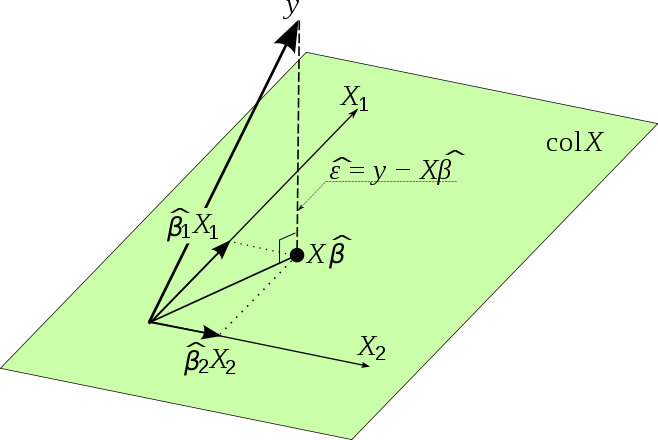
\includegraphics[scale = 0.3]{proj.png}
\end{center}

% talk about what is fatal and what isn't
% freedman, statistical assumptions as empirical commitments
\section{The OLS assumptions}
\begin{list}{$\bullet$}{}

% this is the selection on observables assumption, we can't avoid it, what are we estimating if it isn't right?
\item[1.] \emph{Linear in Parameters}: $Y$ is related to the independent variables and the error term as $Y = X\beta + \epsilon$

% otherwise there is no variation, so we can't actually measure anything
\item[2.] The X's are fixed at take on $\ge$ 2 values
\item[3.] \emph{Full Rank} (in multiple regression): There is no perfect collinearity among any of the independent variables

% otherwise x's aren't exogenous (get endogeneity bias)
\item[4.] \emph{Zero Conditional Mean}: $E(\epsilon | X ) = 0$

% leads to bias... but can be overcome under some assumptions about the variance matrix
\item[5.] \emph{Homoskedasticity}: $Var(\epsilon | X) = \sigma^{2}$

% important for the standard errors... what does it really mean to be iid and random?  Can't have autocorrelation
% 
\item[6.] \emph{Random Sampling}: $Y_{i}$ is an $ iid$ random sample, although this can be relaxed to $cov(y_{i}, y_{j}) = 0 = cov(\epsilon_{i}, \epsilon_{j}) \qquad i \ne j$

% need this for our f-tests and such
\item[7.] \emph{Normal Errors} (optional): $Y \sim \field{N}( X\beta, \sigma^2 ) $
\end{list}

\section{Gauss-Markov Theorem}

\textbf{Gauss-Markov Theorem}: Under assumptions 1-6 above, $\hat{\beta}$ is the best linear unbiased estimator (BLUE) of $\beta$

\subsection{What does BLUE mean?}

% Woolridge
\begin{itemize}
\item[\textbf{B}] est is defined as having the \emph{smallest variance} among the class of linear unbiased estimators
\item[\textbf{L}] inear means that the estimator $\tilde{\beta}$ of $\beta$ is linear $\iff$ it can be expressed as a linear function of the data on the dependent variable
\item[\textbf{U}] nbiased means that $E (\tilde{\beta}) = \beta$
\item[\textbf{E}] stimator is a rule that can be applied to any sample of data to produce an estimate
\end{itemize}

\subsection{The ``U"}
\subsubsection{Unbiasedness of $\hat{\beta}$}
Recall:
%when plugging in Xbeta + epsilon, make sure to say that that is the true model...
\[ \hat{\beta} = (X^{T}X)^{-1}X^{T}Y = (X^{T}X)^{-1}X^{T}(X\beta + \epsilon) = (X^{T}X)^{-1}X^{T}X\beta + (X^{T}X)^{-1}X^{T}\epsilon  = \beta + (X^{T}X)^{-1}X^{T}\epsilon \]

We know that $\hat{\beta}$ is unbiased if $E (\hat{\beta}) = \beta$

\doublespacing
\[ \begin{array}{rl}
E (\hat{\beta}) &= E(\beta + (X^{T}X)^{-1}X^{T}\epsilon | X) \\
 &= E(\beta | X) + E((X^{T}X)^{-1}X^{T}\epsilon | X) \\
 &= \beta + (X^{T}X)^{-1} E(\epsilon | X) \\
 &\qquad \text{where } E(\epsilon | X) = E(\epsilon) = 0 \\
E (\hat{\beta}) &= \beta 
\end{array} \]
\singlespacing


\subsubsection{Unbiasedness of $\hat{\sigma}^2$}

Now, note that:
% what is a trace: sum of diagonal elements of matrix
\doublespacing
\[ \begin{array}{rrl} 
&  E(e^{T}e |X) &= E(\epsilon^{T} \tilde{H} \epsilon | X) \\
& &= E(\sum_{i}\sum_{j} \epsilon_{i} \tilde{H}_{ij} \epsilon_{j} | X) \\ % ei perp ej with E(ei) = 0
& &= \sum_{i} \sum_{j} E(\epsilon_{i} \tilde{H}_{ij} \epsilon_{j} |X ) \\
& & \qquad \text{if } i \ne j, E(\epsilon_{i} \tilde{H}_{ij} \epsilon_{j} |X ) = 0\\
& & \qquad \text{if } i = j, E(\epsilon_{i} \tilde{H}_{ij} \epsilon_{j} |X ) = \sigma^2\tilde{H}_{ii} \\
& &= \sigma^2 Tr(\tilde{H}) \\ %Tr(h~) = Tr(I - H) = Tr(I) - Tr(H) = n - p
& &= \sigma^2 (n - p)
\end{array} \]
\singlespacing

We know that $\hat{\sigma}^2$ is unbiased if $E (\hat{\sigma}^2 |X) = \sigma^2$
\doublespacing
\[ \begin{array}{rl} 
E(\hat{\sigma}^2 | X) &= E(\frac{1}{n-p}e^{T}e | X) \\
 &= \frac{1}{n-p}E(e^{T}e | X) \\
 &= \frac{1}{n-p} \sigma^2 (n - p) \\
 E(\hat{\sigma}^2 | X) &= \sigma^2
\end{array} \]
\singlespacing

\subsection{The ``B''}
We know we want an estimator of the form $\tilde{\beta} = m + MY$ with $E(\tilde{\beta} | X) = \beta$
\[ E(\tilde{\beta} | X) = E(m + MY | X) = E(m + M(X\beta + \epsilon) | X) = m + MX\beta \]
\begin{equation} \Rightarrow m = 0 \text{ and }MX = I_{p \times p} \end{equation}
Therefore, this implies we want $\tilde{\beta} = MY$, so WLOG we can say $M = (X^{T}X)^{-1}X^{T} + c$

Thus,
\[ MX = ((X^{T}X)^{-1}X^{T} + c)X = X^{T}X)^{-1}X^{T}X + cX = I_{p \times p} + CX  = I_{p \times p} \text{ by (1)} \]
\begin{equation} \Rightarrow CX = 0 \end{equation}

Also note that
\[ \tilde{\beta} = MY = M(X\beta + \epsilon) = \beta + M\epsilon \text{ by } MX = I_{p \times p} \]
\begin{equation} \Rightarrow \tilde{\beta} - \beta = M\epsilon \end{equation}

Now, as noted in section 3.1, ``best'' means having the smallest variance, therefore we want to minimize $cov(\tilde{\beta} | X)$

\doublespacing
\[ \begin{array}{rl}
cov(\tilde{\beta} | X) &= E((\tilde{\beta} - \beta)(\tilde{\beta} - \beta)^{T} | X) \\
&= E((M\epsilon)(M\epsilon)^{T} |X) \\
&= E(M\epsilon \epsilon^{T} M^{T} |X) \\
&= M E(\epsilon \epsilon^{T} | X) M^{T} \\
&= \sigma^2MM^{T}
\end{array} \]
\singlespacing

where,
\doublespacing
\[ \begin{array}{rl}
MM^{T}  &= \big((X^{T}X)^{-1}X^{T} + c\big)\big((X^{T}X)^{-1}X^{T} + c\big)^{T} \\
&= (X^{T}X)^{-1}X^{T}X(X^{T}X)^{-1} + (X^{T}X)^{-1}X^{T}C^{T} + CX(X^{T}X)^{-1} + CC^{T} \\
& \qquad \text{ where, from (2), } CX = 0 \text{ and } C^{T}X^{T} = 0 \\
MM^{T} &= (X^{T}X)^{-1} + CC^{T}
\end{array} \]
\singlespacing

Thus,
\[ cov(\tilde{\beta} | X) = \sigma^2(X^{T}X)^{-1} + \sigma^2CC^{T} \]

$MM^{T}$ is variance matrix of the estimator, and it is minimized when $CC^{T}$ = 0.  Therefore, any estimator besides $\hat{\beta}$ has strictly greater variance because only $\hat{\beta}$ will have $CC^{T} = 0$.

Finally, we get that the ``best'' estimator is where $C = 0$, thus getting
\[ \tilde{\beta} = (X^{T}X)^{-1}X^{T}Y = \hat{\beta} \]

% W&M 160
\section{The Sherlock Holmes approach to Regression}

How do you decide what to put into the model?

\begin{itemize}
\item Say that you have a theoretical reason to believe your model is correctly specified.  Then, that should only leave measurement, sampling, and observation challenges.
\begin{itemize}
% example, hooke's law works
\item Weakness: Critics will claim that your model is wrong, that some number of variables are or are not included, and it is hard to say that they are wrong in the social sciences
\end{itemize}
\item Then, since theoretical reasons for including covariates may not be enough, one can ask: ``Can the \emph{data} generate an all-cause, complete specification (i.e. correctly specified) model?"
\item Leamer's (1978) ``The Axiom of Correct Specification"
\begin{itemize}
\item[a] The set of explanatory variables that are thought to determine (linearly) the dependent variable must be (1) unique, (2) complete, (3) small in number, and (4) observable.
\item[b] Other determinants of the dependent variable must have a probability distribution with at most a few unknown parameters
\item[c] All unknown parameters must be constant
\end{itemize}

\item However, Leamer immediately turns around to say:
\begin{quote}
``If this axiom were, in fact, accepted, we would find one equation estimated for every phenomenon, and we would have books that compiled these estimates published with the same scientific fanfare that accompanies estimates of the speed of light or the gravitational constant.  Quite the contrary, we are literally deluged with regression equations, all offering to ``explain'' the same event, and instead of a book of findings we have volumes of competing estimates.''
\end{quote}

\item Instead, most regressions are produced using ``data-instigated specification search'', or the ``Sherlock Holmes'' approach.
\begin{itemize}
\item Instead of using a theoretical based model, a lot of times people will include some covariates because they are available, some because they have a theoretical basis, even some post-treatment variables
\item Very often, then, people run the regression, see what is significant or not (especially the variables of interest), then either remove or add more covariates to change the standard errors
\end{itemize}

\item Leamer's response is that this approach is terrible
\begin{quote}
`` $\dots$ if theories are constructed after having studied the data, it is difficult to establish by how much, if at all, the data favor the data-instigated hypothesis.  For example, suppose I think that a certain coefficient ought to be positive, and my reaction to the anomalous result of a negative estimate is to find another variable to include in the equation so that the estimate is positive.  Have I found evidence that the coefficient is positive?'' (1983)
\end{quote}

\item There are new approaches to data-mining that avoid some of these pitfalls, but it is still a tricky business.
\end{itemize}
\end{document}